\section{Opgave 2: Binary to Decimal Conversion}
\begin{enumerate}
	\item[1)]
	Vi har læst koden for BCD decoderen og er indforstået med hvad der fungerer hvordan, og hvorfor.\newline
	
	\item[2)]
	Vi skriver koden for en 7-segment decoder ved hjælp af with/select i VHDL:\\
		\begin{lstlisting}[caption={BCD til 7 segment decoder},label={lst:bcdTo7SegDecoder}]
		library ieee;
		use ieee.std_logic_1164.all;
		
		entity BCDdecoder is
		port(dcba: in std_logic_vector(3 downto 0);
		seg: out std_logic_vector(6 downto 0));
		end BCDdecoder;
		
		architecture selection of BCDdecoder is
		begin
		with dcba select
		seg<="0000001" when "0000",
		"1001111" when "0001",
		"0010010" when "0010",
		"0000110" when "0011",
		"1001100" when "0100",
		"0100100" when "0101",
		"1100000" when "0110",
		"0001111" when "0111",
		"0000000" when "1000",
		"0001100" when "1001",
		"1111111" when others;
		end selection;	
		\end{lstlisting}
		
\item[3)]
	Vi tester programmet på DE2-boardet. Vi bruger SW[3:0] som input og HEX0 som output. Vi tester først med 0 som input og får forventet output som ses på figur \ref{fig:7SegDecoder0}:
	\begin{figure}[h]
		\centering
		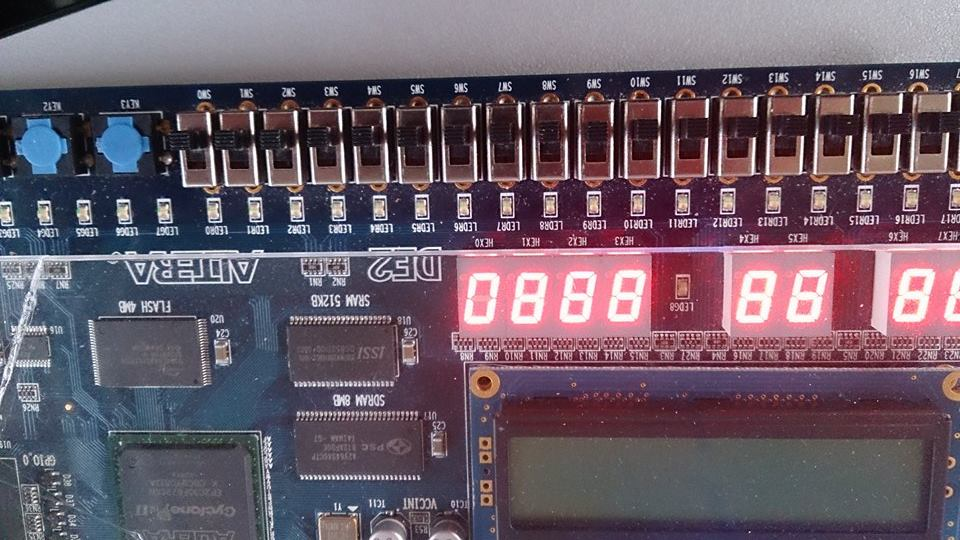
\includegraphics[scale=0.6]{pictures/Oevelse4/BCD_decoder/BCD_1seg_0.jpg}
		\caption{7-segment decoder med 0 som input}
		\label{fig:7SegDecoder0}
	\end{figure}

Vi tester nu med 9 som input og får forventet output som ses på figur \ref{fig:7SegDecoder9}:
\begin{figure}[h]
	\centering
	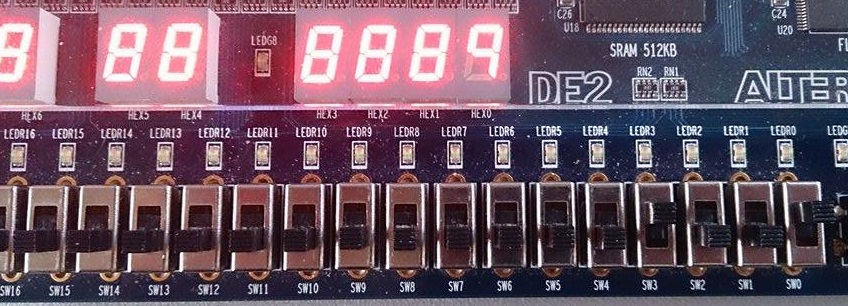
\includegraphics[scale=0.6]{pictures/Oevelse4/BCD_decoder/BCD_1seg_9.jpg}
	\caption{7-segment decoder med 9 som input}
	\label{fig:7SegDecoder9}
\end{figure}

Vi tester nu med ugyldigt input (over 9) og får som forventet blankt output som ses på figur \ref{fig:7SegDecoderUgyldig}:
\begin{figure}[h]
	\centering
	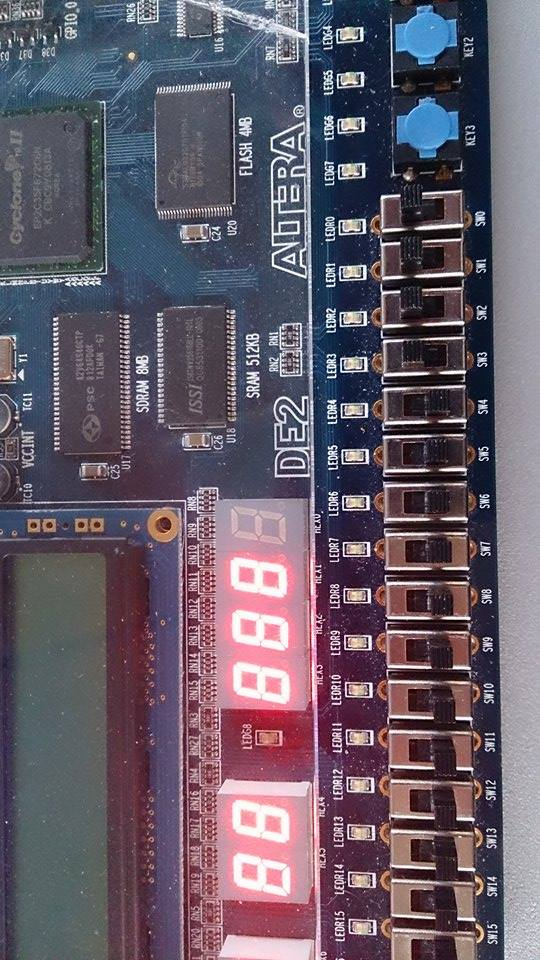
\includegraphics[scale=0.6]{pictures/Oevelse4/BCD_decoder/BCD_1seg_ugyldig.jpg}
	\caption{7-segment decoder med ugyldigt input}
	\label{fig:7SegDecoderUgyldig}
\end{figure}

\item[4)]
	Vi skriver koden for en to-segments decoder ved hjælp af when-statements, som ses i kode  \ref{lst:bcdToTwo7SegDecoder}
			\begin{lstlisting}[caption={BCD til to 7 segment decoder},label={lst:bcdToTwo7SegDecoder}]
			library ieee;
			use ieee.std_logic_1164.all;
			use ieee.numeric_std.all;
			
			entity TwoDigitDecoder is
			port(V: in std_logic_vector(3 downto 0);
			seg1, seg10: out std_logic_vector(6 downto 0));
			end TwoDigitDecoder;
			
			architecture selection of TwoDigitDecoder is
			signal M, X: std_logic_vector(3 downto 0);
			signal Z: std_logic ;
			
			begin
			Z <= '1' when(V > "1001") else '0';
			M <= V when(Z = '0') else (std_logic_vector(unsigned(V) - 10));  
			X <= "000" & Z;
			
			seg1<="0000001" when (M = "0000") else
			"1001111" when (M = "0001") else
			"0010010" when (M = "0010") else
			"0000110" when (M = "0011") else
			"1001100" when (M = "0100") else
			"0100100" when (M = "0101") else
			"1100000" when (M = "0110") else
			"0001111" when (M = "0111") else
			"0000000" when (M = "1000") else
			"0001100" when (M = "1001") else
			"0000001" when (M = "1010") else
			"1001111" when (M = "1011") else
			"0010010" when (M = "1100") else
			"0000110" when (M = "1101") else
			"1001100" when (M = "1110") else
			"0100100" when (M = "1111") else "1111111";
			
			seg10<="0000001" when (X = "0000") else
			"1001111" when (X = "0001") else "1111111";
			
			end selection;
			\end{lstlisting}
	
\end{enumerate}